\section*{Aufgabe 7.1a)}
In der ersten Teilaufgabe sollte für das Potential
\begin{eqnarray}
V(x) = V_0 \Theta(ω-|x|)\left[ 1-\frac{|x|^n}{ω} \right]
\end{eqnarray}
die Streuphasen $δ_{\pm}$ berechnet und geplottet werden. Der dafür geschriebene
Code ist in \lref{streuung} dargestellt, die darin aufgerufene Funktion \texttt{ho\_fou}
ist in \lref{ho_fou} zu sehen.

\lstinputlisting[label=lst:streuung,caption={streuung.m}]{../code/streuung.m}
\lstinputlisting[label=lst:ho_fou,caption={ho\_fou.m}]{../code/ho_fou.m}

Es resultieren hierbei Plots für die drei zu verwendenden Werte von $n$, die wie
folgt dargestellt sind:
\begin{itemize}
\item für $n=1$ für \fref{n1}
\item für $n=2$ für \fref{n2}
\item für $n=10$ für \fref{n10}.
\end{itemize}

\begin{figure}[htb]
  \centering
  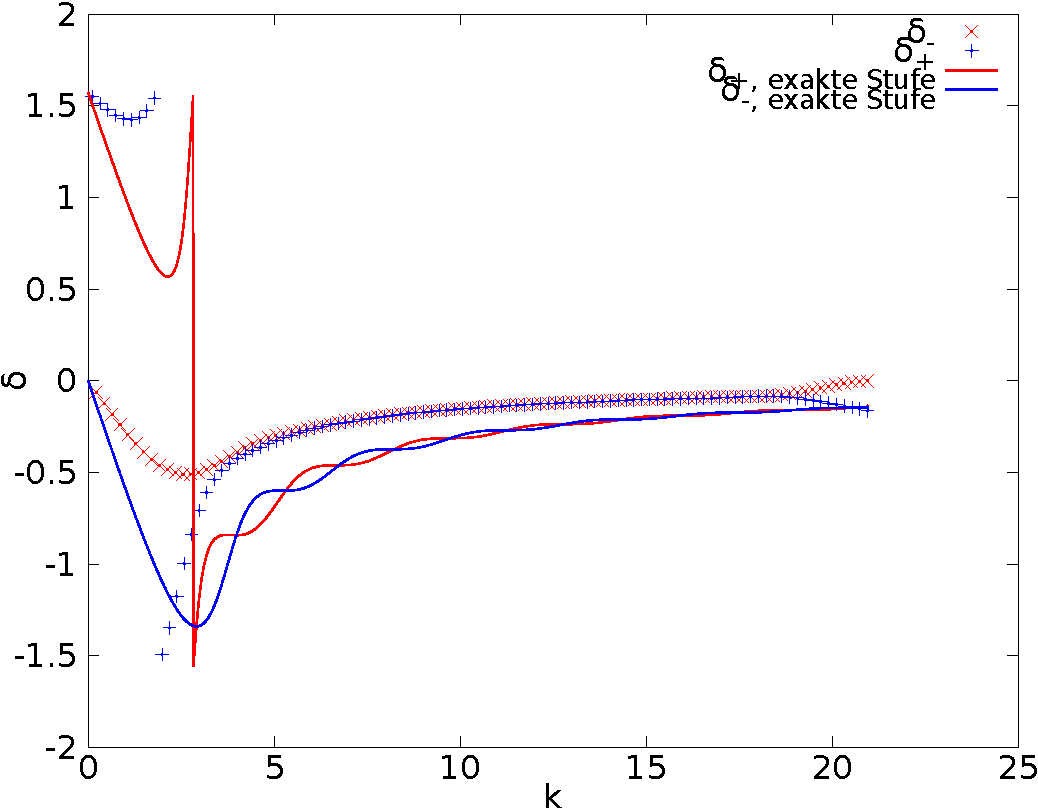
\includegraphics[width=0.8\columnwidth,keepaspectratio]{../tmp/71a_n1-crop}
  \caption{Streuphasen für $n=1$, }
  \label{fig:n1}
\end{figure}

\begin{figure}[htb]
  \centering
  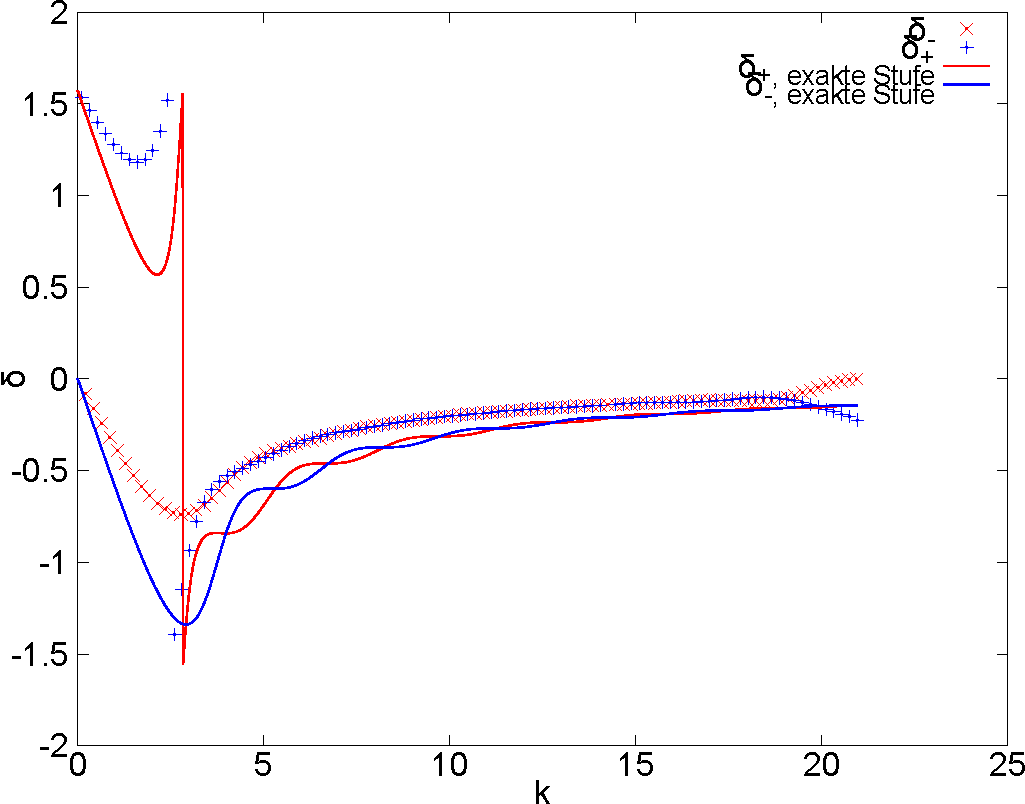
\includegraphics[width=0.8\columnwidth,keepaspectratio]{../tmp/71a_n2-crop}
  \caption{Streuphasen für $n=2$, }
  \label{fig:n2}
\end{figure}

\begin{figure}[htb]
  \centering
  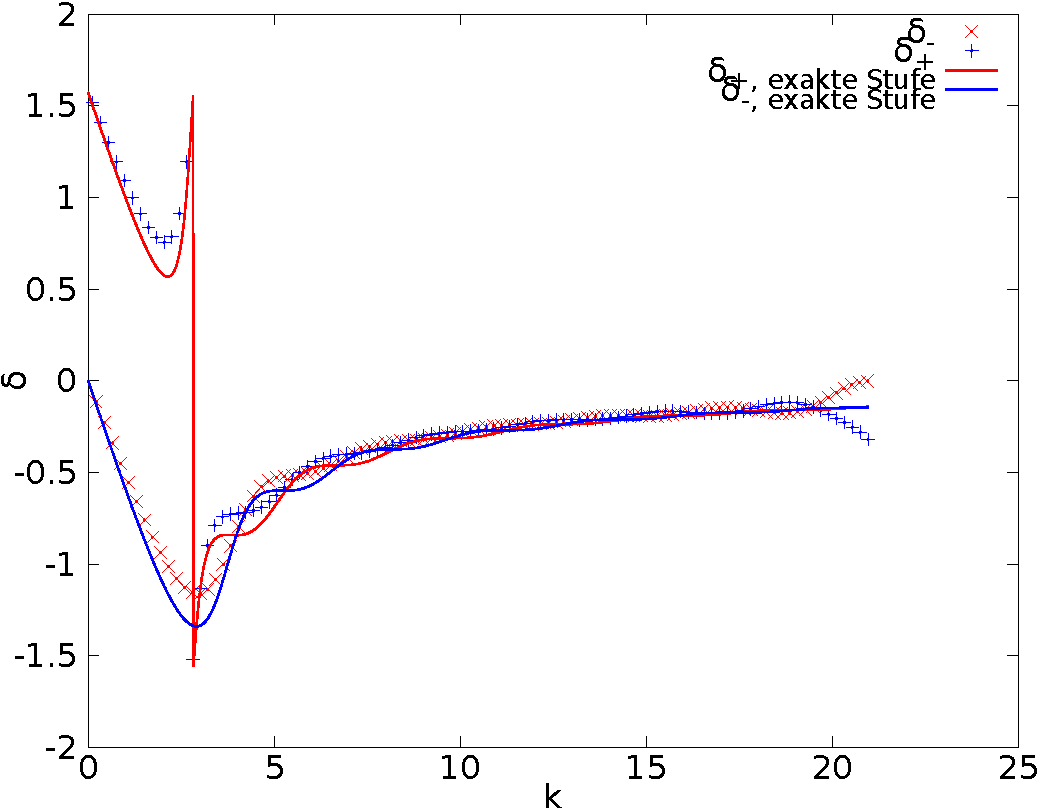
\includegraphics[width=0.8\columnwidth,keepaspectratio]{../tmp/71a_n10-crop}
  \caption{Streuphasen für $n=10$, }
  \label{fig:n10}
\end{figure}

Wie man erkennen kann, stimmen für größer werdende $n$, also für immer rechteckigere
Potentiale, die exakten Lösungen und die numerische Lösung besser überein.

\section*{Aufgabe 7.1b)}
In diesem Teil der Aufgabe wird die Born'sche Näherung untersucht. Die Formel, an
der sich orientiert wurde, stammt aus dem Skript.
\begin{eqnarray}
δ_+ &=& -\frac{2}{k}\int\limits_0^ω\dd{x}V(x)\cos^2(kx)\\
&=& -\frac{2 V_0}{k}\int\limits_0^ω\dd{x}(1-\frac{x}{ω})\cos^2(kx)\\
&=& \frac{V_0}{4k^3 ω} \left(-1 + \cos(2kω) - 2k^2 ω^2\right)\\
δ_- &=& -\frac{2}{k}\int\limits_0^ω\dd{x}V(x)\sin^2(kx)\\
&=& \frac{V_0}{4k^3 ω} \left(1 - \cos(2kω) - 2k^2 ω^2\right)
\end{eqnarray}
Die Integration wurde mit Hilfe des analytisch rechnenden Open-Source-Programms
\texttt{Maxima} durchgeführt. Die erhaltenen Lösungen wurden in der nächsten
Aufgabe implementiert.

\section*{Aufgabe 7.1c)}
Der entsprechende Code für die Implementierung ist im Wesentlichen in \lref{streuung}
in den Zeilen \textcolor{red}{51 bis 57} zu finden. Daraus resultiert der Plot in \fref{1c}.

\begin{figure}[htb]
  \centering
  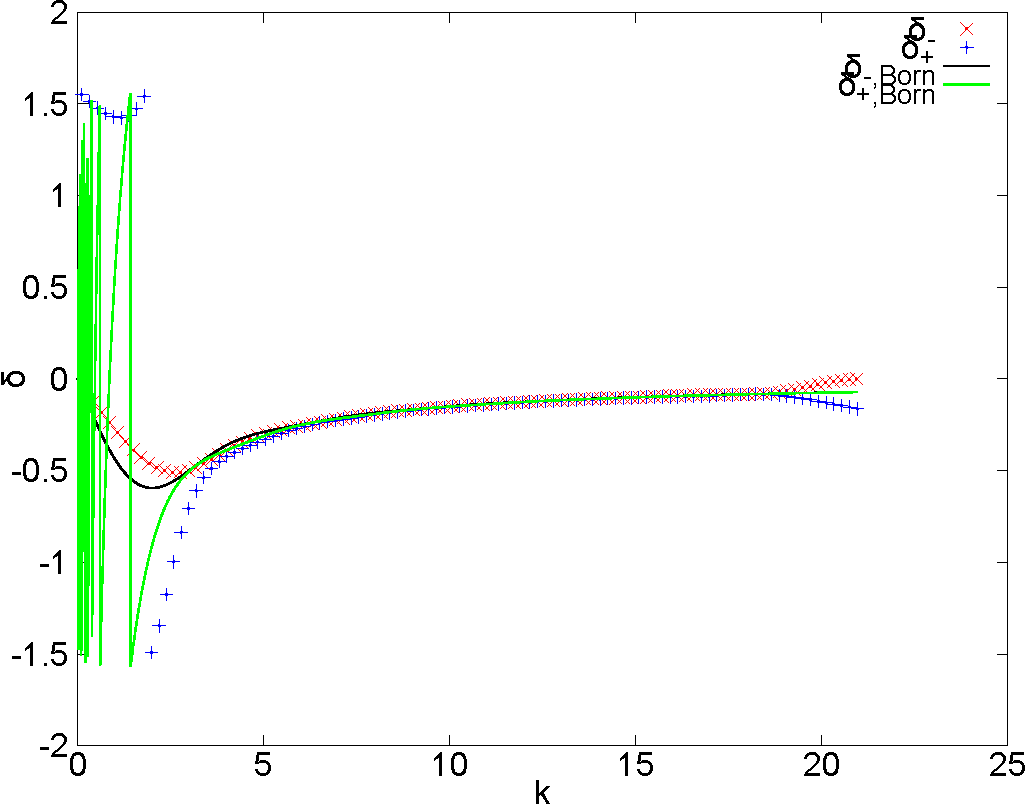
\includegraphics[width=0.8\columnwidth,keepaspectratio]{../tmp/71c-crop}
  \caption{Vergleich der exakten Lösungen der Streuphasen mit den nummerisch
  berechneten für $n=1$}
  \label{fig:1c}
\end{figure}

Wie man erkennen kann, stimmen die Born'sche Näherung und die in a) berechnete
nummerische Lösung für etwa $5<k<20$ gut überein, während für kleinere $k$ die
Born'sche Näherung für gerade Paritäten noch annähernd wie die nummerische Lösung
verläuft, aber für ungerade Paritäten ein unphysikalisches Verhalten aufweist (starkes
Schwanken bei geringer $k$-Änderung).

\section*{Aufgabe 7.1d)}
In der letzten Teilaufgabe sollte die numerische Lösung für das Dreieckspotential
mit der exakten für ein Stufenpotential verglichen werden, wobei die Integrale über
beide Potentiale gleich sein sollten. Daher wurde die Höhe des Stufenpotentials auf
die Hälfte reduziert, sodass die Fläche des Stufenpotentials der des Dreieckspotentials
entspricht. Wenn die Potentiale modifiziert werden, dann ergibt sich der in \fref{1d}
dargestellte Plot.

\begin{figure}[htb]
  \centering
  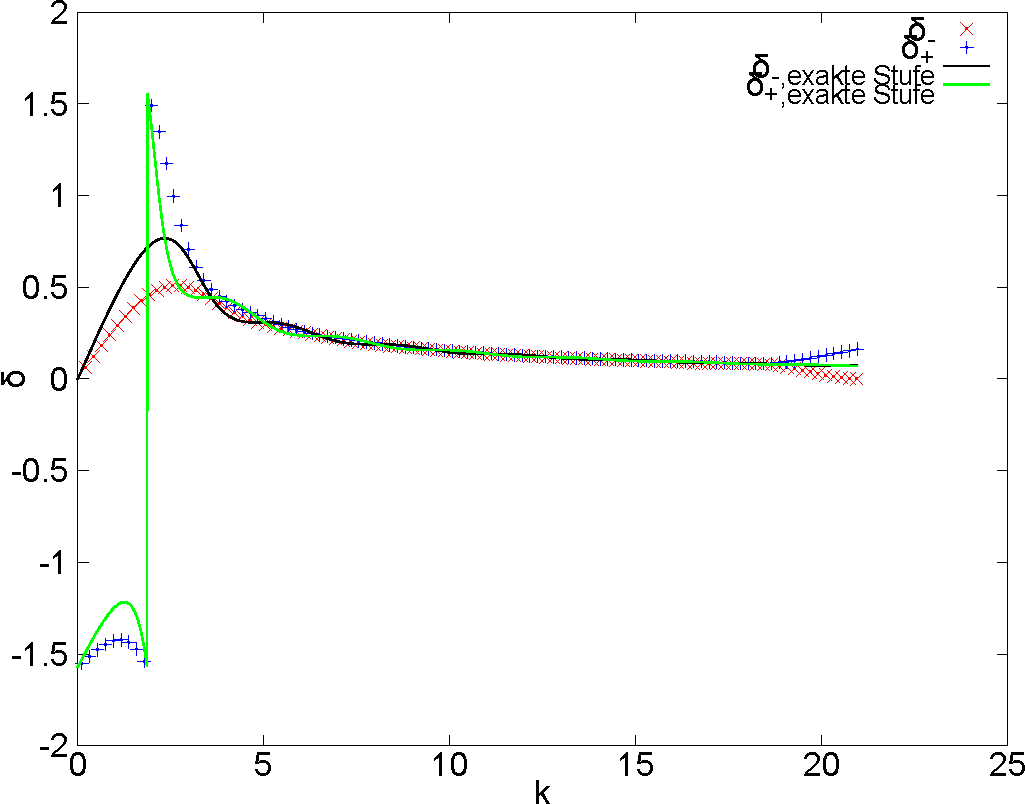
\includegraphics[width=0.8\columnwidth,keepaspectratio]{../tmp/71d-crop}
  \caption{Vergleich der nummerischen Lösungen der Streuphasen für $n=1$ mit denen für eine
  exakte Potentialstufe}
  \label{fig:1d}
\end{figure}
Integral 